%-----------------------------------------------
% Template para criação de resumos de projectos/dissertação
% jlopes AT fe.up.pt,   Fri Jul  3 11:08:59 2009
%-----------------------------------------------

\documentclass[9pt,a4paper]{extarticle}

%% English version: comment first, uncomment second
\usepackage[portuguese]{babel}  % Portuguese
%\usepackage[english]{babel}     % English
\usepackage{graphicx}           % images .png or .pdf w/ pdflatex OR .eps w/ latex
\usepackage{times}              % use Times type-1 fonts
\usepackage[utf8]{inputenc}     % 8 bits using UTF-8
\usepackage{url}                % URLs
\usepackage{multicol}           % twocolumn, etc
\usepackage{float}              % improve figures & tables floating
\usepackage[tableposition=top]{caption} % captions
%% English version: comment first (maybe)
%\usepackage{indentfirst}        % portuguese standard for paragraphs
%\usepackage{subfig}
%\usepackage{todonotes}
%\usepackage{parskip}

%% page layout
\usepackage[a4paper,margin=30mm,noheadfoot]{geometry}

%% space between columns
\columnsep 12mm

%% headers & footers
\pagestyle{empty}

%% figure & table caption
\captionsetup{figurename=Fig.,tablename=Tab.,labelsep=endash,font=bf,skip=.5\baselineskip}

%% heading
\makeatletter
\renewcommand*{\@seccntformat}[1]{%
  \csname the#1\endcsname.\quad
}
\makeatother

%% avoid widows and orphans
\clubpenalty=300
\widowpenalty=300

\begin{document}

\title{\vspace*{-8mm}\textbf{\textsc{Programação por utilizadores finais em dispositivos móveis através da re-utilização de componentes visuais compostos}}
\author{\emph{Tiago Manuel da Silva Almeida}\\[2mm]
\small{Dissertação realizada sob a orientacão do \emph{Prof.\ Hugo Sereno Ferreira}}\\
\small{e co-orientada por Tiago Boldt Sousa}}}
\date{}
\maketitle
%no page number 
\thispagestyle{empty}

\vspace*{-4mm}\noindent\rule{\textwidth}{0.4pt}\vspace*{4mm}

\begin{multicols}{2}

\section{Motivação}\label{sec:motiva}

As vendas de \emph{smartphones} ultrapassaram as vendas de PCs, e, consequentemente, o numero de utilizadores finais de smartphones crescem. Os utilizadores finais exigem aplicações customizáveis em quantidade para os seus dispositivos. Esta exigência faz com que seja impraticável para um desenvolvedor de software prever todas as alternativas válidas.

Uma possível solução para fazer aplicações costumizáveis passa por criar ferramentas que usam \emph{programação por utilizadores finais} (PUF).
PUF é ``a escrita de programas de computador por parte de um utilizador final para satisfazer uma necessidade específica, mas a programação não é o trabalho principal deste utilizador final''~\cite{EUSEReport}.
Essa ferramenta poderia ser uma framework colaborativa, onde novatos e experientes poderiam partilhar e coexistir, enquanto os utilizadores finais exploram os seus requisitos.
Com este cenário, utilizadores experientes poderiam criar componentes que podiam ser ligados por utilizadores finais recorrendo uma linguagem de programação visual (LPV).
Esta ferramenta poderia reduzir o número de pequenas aplicações desenhadas para um problema muito específico, mas também poderiam impulsionar a descoberta e experiencias dos utilizadores finais.

\section{Objectivos}\label{sec:goals}

Os nossos objetivos passam por responder aos seguintes problemas, usando um protótipo funcional:

\begin{itemize}
	\item{\textbf{Limitações de um smartphone na implementação de uma solução que usa PUF} 
	LPVs podem ser impraticáveis em ecrãs pequenos. Como podemos usar elementos visuais sem sobrecarregar o ecrã? Uma solução típica que usa um esquema de \emph{data-flow} com zoom é suficiente? Podemos usar LPVs num ecrã pequeno
	e mesmo assim trabalhar com soluções com um numero medio/grande de componentes?}

	\item{\textbf{Definição de um nível de abstração para uma \emph{framework} colaborativa} 
	Altos níveis de abstração podem ser bons para utilizadores finais, mas podem limitar os blocos produzidos por programadores experientes. Podemos atingir um nivel de abstração equilibrado para os utilizadores finais e programadores experientes?}
  
	\item{\textbf{Reutilização de blocos em PUF} 
	Como podemos reutilizar componentes e incentivar os utilizadores finais a reutilizar? É possível beneficiar de um plataforma de partilha de componentes? Existem outras formas de reutilização?}
	
\end{itemize}

\section{De Android a Scala: Passos numa Solução que usa PUF} \label{sec:work}

Inicialmente olhamos para a os problemas da PUF~\cite{Barriers2004}, que rapidamente nos consciencializou noutro tópico: \emph{Engenharia de Software para Utilizadores Finais} (ESUF). Adicionalmente, descobrimos que as LPVs são uma forma de resolver esses problemas~\cite{Navarro2001} e estudamos as suas propriedades. Com o conhecimento adquirido, desenvolveu-se um protótipo para Android recorrendo a conceitos das LPVs. Esse protótipo foi melhorado de acordo com o \emph{feedback} dos utilizadores finais através de experiencias informais.
Nestes testes, um dos problemas mais comuns era o elevado número de blocos necessário para realizar tarefas simples. Para resolver este problema pensamos num sistema de regras de reescrita e decidimos experimentar uma nova linguagem para o fazer: Scala~\cite{ProgrammingScala}.


\subsection{Protótipo Tipado Baseado em Blocos}

\begin{figure}[H]
\centerline{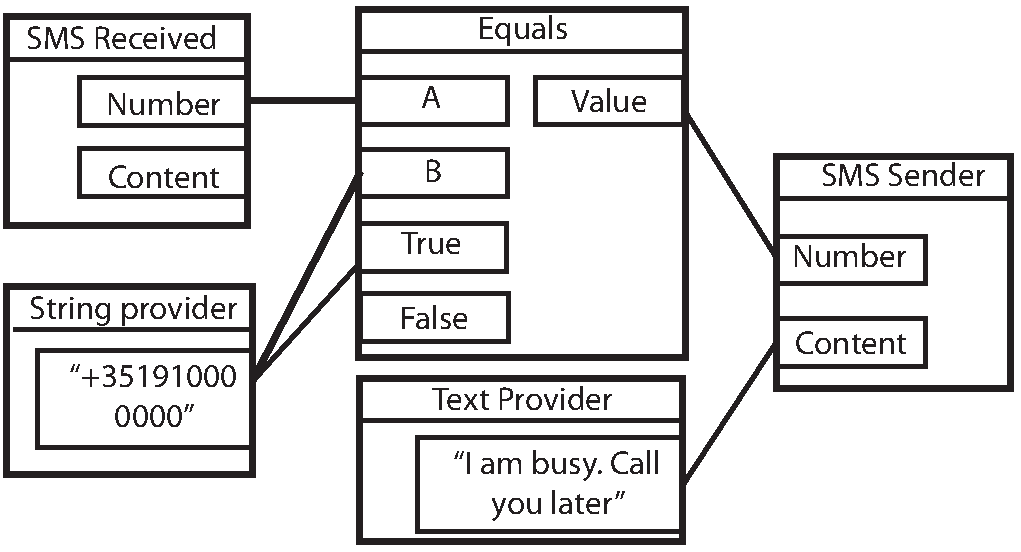
\includegraphics[scale=.40]{block_example.pdf}}
\caption{Uma tarefa composta por um conjunto de blocos.} 
\label{fig:block}
\end{figure}

Representar uma função ou algoritmo como um bloco, com entradas e saídas, já foi usado na engenharia de \emph{software} (por exemplo, os testes de caixa-preta~\cite{BlackBoxTesting}). Esta metáfora dos blocos também já foi pensada para usar em PUF ~\cite{Zin2011}. Chamamos às saídas e entradas de conectores e cada conector tem um tipo. As saídas podem ligar a entradas e um conjunto de blocos ligados constitui outro bloco que pode ser reutilizado.

Um bloco pode ser mostrado a um utilizador final usando uma caixa com entradas na esquerda e saídas na direita. Os blocos podem ser desenvolvidos por programadores experientes e os utilizadores finais podem liga-los. Um conjunto de blocos ligados define uma tarefa e uma tarefa, é, ela mesma, um bloco que pode ser ligado com outros blocos e criar novas tarefas.

A figura \ref{fig:block} mostra uma tarefa que responde automaticamente a uma mensagem recebida com o conteúdo ``I am busy. Call you later'' quando a mensagem recebida foi enviada pelo numero ``+351910000000''. O bloco com o nome ``equal''
tem dois conjuntos de entradas: \texttt{A} e \texttt{B}, que são os valores que vão ser comparados; \texttt{True} e \texttt{False}, que são os valores a usar no caso da expressão \texttt{A == B} ser verdadeira ou falsa. 
A saída com o nome \texttt{Value} terá o valor das entradas \texttt{True} ou \texttt{False} dependendo do resultado da expressão.

As tarefas podem ser criadas no protótipo através de duas colunas expansíveis. Inicialmente só existe duas colunas no ecrã que podem ser usadas para adicionar blocos. Se o utilizador quiser ligar blocos aos blocos da coluna da direita ele pode fazer um \emph{swipe} da direita para a esquerda. Com este gesto, os blocos da coluna da direita passam para a esquerda e uma nova coluna vazia aparece na direita.

\subsection{Experiencias com um Sistema de Regras de Reescrita}

O \emph{feedback} dos utilizadores finais permitiu algumas melhorias mas deixou duas propostas pendentes: simplificação automática num conjunto de blocos e conversão dos tipos dos conectores sem recorrer a blocos extra. Para resolver estes problemas tentamos usar Scala, que possui duas funcionalidades úteis: \emph{pattern matching} e \emph{implicit conversions}. \emph{Pattern matching} permite a procura de padrões num conjunto de blocos ligados de uma forma fácil. \emph{Implicit convertions} possibilita a definição de algumas conversões sem a necessidade de fazer \emph{cast} ou usar funções de conversão nos tipos dos conectores. Em Java, se quiséssemos converter de uma \texttt{String} para um \texttt{Integer} poderíamos fazer: \texttt{Integer.parseInt(string)}. Em Scala é possível definir uma \emph{implicit conversion} e toda a vez que uma \texttt{String} é usada e um \texttt{Integer} é esperado, a conversão é automaticamente realizada.

Usando pattern matching construi-se um sistema de regras de reescrita para simplificar automaticamente situações como: quando um conjunto de blocos tem duas contantes que estão a ser somadas, então substitui por uma constante. Em níveis mais baixos não há uma substituição no comportamento do sistema, em vez da substituição é fornecida uma abstração visual.

\section{Conclusions and Future Work}\label{sec:conclui}

Nós não conseguimos usar o sistema de regras de reescrita devido à fase precoce em que Scala se encontra no que diz respeito à compilação para Android. Até à data, Scala para Android tinha como problemas principais a compilação lenta e problemática. No entanto, o nosso protótipo em Java está completamente funcional, permitindo a adição de novos blocos por parte dos utilizadores experientes e a composição dos mesmos por parte dos utilizadores finais.
Desta forma, os utilizadores finais podem construir tarefas customizadas que são uteis para as suas atividades diárias. No entanto, estes dispositivos têm um tamanho reduzido de ecrã, então tivemos de fornecer uma solução escalável que divide a composição horizontalmente.

O \emph{feedback} recolhido dos utilizadores finais permitiu-nos entender quais as suas prioridades e necessidades, permitindo-nos perceber que os utilizadores finais preferem tarefas com poucos blocos. Também observamos que facilmente não se percebia como se criava uma tarefa na primeira utilização, mas uma explicação oral era suficiente para eles começarem. Então, incluímos um pequeno tutorial no protótipo que explica o processo de criação de tarefas.

Como parte do trabalho futuro tencionamos fazer experiencias formais com utilizadores finais para validar a nossa implementação. Para isso, vamos fornecer aos utilizadores finais um guião que deverá ser seguido, de forma a medir a habilidade com que cada utilizador final faz cada passo, considerando o tempo, intuitividade, erros cometidos e comentários. Um questionário final fornecerá \emph{feedback} das opiniões dos utilizadores finais em relação à aplicação. Essa informação será relevante para entender os defeitos de usabilidade na aplicação. Após atingirmos a maturidade desejada na aplicação tencionamos publica-la no \emph{Android market}. As futuras versões poderão incluir partilha de blocos (e tarefas) entre utilizadores como forma de extensões que poderão ser transferidas dentro da aplicação.


%%English version: comment first, uncomment second
\bibliographystyle{unsrt-pt}  % numeric, unsorted refs
%\bibliographystyle{unsrt}  % numeric, unsorted refs
\bibliography{refs}

\end{multicols}

\end{document}
